\subsection{DHT22 -- Sensor Suhu \& Kelembapan Udara}
\label{subsec:dht22}

% ---------------------------------------------------------------------
\subsubsection{Identitas dan Fungsi}
DHT22 (AM2302) adalah modul sensor digital yang berfungsi untuk mengukur suhu dan kelembapan relatif (\textit{relative humidity}) secara simultan. Modul ini dipilih karena menawarkan rentang pengukuran yang luas, akurasi tinggi dengan kompensasi suhu penuh, serta antarmuka digital kustom \textit{1-wire bus} yang efisien dalam penggunaan pin I/O mikrokontroler.

\begin{table}[H]
	\centering
	\caption{Identitas komponen DHT22 / AM2302}
	\label{tab:dht22_identitas}
	\small
	\begin{tabularx}{\textwidth}{@{}lX@{}}
		\toprule
		Parameter          & Keterangan                                                                    \\
		\midrule
		Nama komponen      & AM2302 / DHT22                                                                \\
		Model/part number  & AM2302 Digital Relative Humidity and Temperature Sensor                       \\
		Jenis              & Sensor Digital (Kombinasi Suhu dan Kelembapan)                                \\
		Fungsi utama       & Mengukur temperatur udara dan kelembapan relatif (\textit{Relative Humidity}) \\
		Sumber dokumentasi & AM2302 Datasheet (Adafruit)                                                   \\
		\bottomrule
	\end{tabularx}
\end{table}

% ---------------------------------------------------------------------
\subsubsection{Prinsip Kerja}
Di dalam modul DHT22 (AM2302), komponen penyusunnya terbagi pada dua sisi papan rangkaian internal. Sisi depan memuat \textit{NTC thermistor} dan elemen sensoris kelembapan, sedangkan sisi belakang memuat mikrokontroler 8-bit internal yang menangani akuisisi data, pemrosesan, dan transmisi sinyal melalui protokol digital \textit{1-Wire}.

DHT22 mengukur parameter lingkungan melalui dua elemen sensoris utama:

\begin{enumerate}
	\item \textbf{Elemen Suhu (\textit{NTC Thermistor}):}
	      Pengukuran temperatur ditangani oleh \textit{Negative Temperature Coefficient} (NTC) \textit{thermistor}, yaitu komponen resistor yang memiliki hubungan berbanding terbalik dengan suhu. Nilai resistansi NTC akan menurun secara eksponensial saat suhu meningkat dan sebaliknya. Mikrokontroler internal membaca resistansi NTC ini dan menghitung nilai suhu yang sesuai menggunakan kurva karakteristik NTC sebelum dikonversi menjadi data digital.

	      \begin{figure}[H]
		      \centering
		      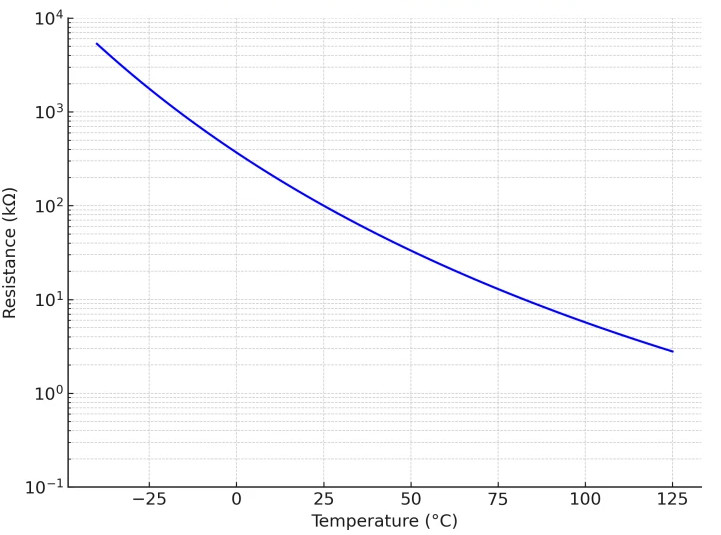
\includegraphics[width=0.50\textwidth]{images/ntc_char.jpg}
		      \caption{Kurva karakteristik hubungan suhu terhadap resistansi pada NTC Thermistor.}
		      \label{fig:ntc_karakteristik}
	      \end{figure}

	\item \textbf{Elemen Kelembapan (Kapasitor Peka Kelembapan):}
	      Pengukuran kelembapan memanfaatkan komponen kapasitor peka kelembapan (\textit{moisture-sensitive capacitor}) yang nilai kapasitansinya berubah sesuai dengan tingkat kelembapan udara. Mikrokontroler internal mengisi dan mengosongkan muatan (\textit{charging/discharging}) pada kapasitor tersebut untuk menentukan nilai kapasitansinya berdasarkan durasi waktu pengisian/pengosongan, lalu mengonversinya menjadi sinyal digital Kelembapan Relatif (\textit{Relative Humidity}/RH).

	      \begin{figure}[H]
		      \centering
		      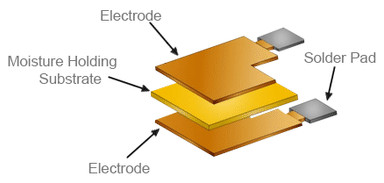
\includegraphics[width=0.50\textwidth]{images/humid_internal.jpg}
		      \caption{Komponen internal elemen sensoris kelembapan pada DHT22.}
		      \label{fig:humidity_capacitor}
	      \end{figure}

\end{enumerate}

\paragraph{Konsep dan Formulasi Kelembapan Relatif (RH)}
Kelembapan Relatif ($RH$) merupakan rasio jumlah uap air aktual di udara dibandingkan dengan jumlah maksimum uap air yang dapat ditampung oleh udara pada suhu tertentu. Formulasi matematikanya dinyatakan sebagai:

\begin{equation}
	RH = \frac{\rho_w}{\rho_s} \times 100\%
	\label{eq:dht22_rh}
\end{equation}

\noindent di mana:
\begin{itemize}
	\item $RH$ = Kelembapan Relatif (\%).
	\item $\rho_w$ = Densitas uap air aktual pada suhu tertentu ($\text{g/m}^3$).
	\item $\rho_s$ = Densitas uap air pada kondisi jenuh pada suhu yang sama ($\text{g/m}^3$).
\end{itemize}

Kapasitas udara dalam menampung uap air dipengaruhi oleh suhu; udara dingin memiliki kapasitas titik jenuh yang lebih rendah, sedangkan udara panas dapat menampung uap air lebih tinggi sebelum mencapai titik jenuh. Ketika $RH = 100\%$, udara berada pada kondisi jenuh total sehingga terjadi kondensasi (embun), sedangkan $RH = 0\%$ menunjukkan kondisi udara kering sempurna.

Sinyal analog yang diproses oleh mikrokontroler internal dikompensasi secara penuh berdasarkan koefisien kalibrasi presisi pada memori OTP (\textit{One-Time Programmable}) sebelum ditransmisikan.

\begin{figure}[H]
	\centering
	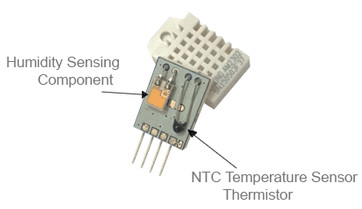
\includegraphics[width=0.75\textwidth]{images/dht22_block.jpg}
	\caption{Elemen sensoris AM2302/DHT22.}
	\label{fig:dht22_sensoris_elemen}
\end{figure}


\subsubsection{Alur Kerja Internal dan Protokol Komunikasi}

Alur pemrosesan data internal sensor DHT22 mengikuti pola \textbf{Input $\rightarrow$ Proses $\rightarrow$ Output}:
\begin{enumerate}
	\item \textbf{Input:} Perubahan kelembapan udara mengubah nilai kapasitansi elemen polimer, sedangkan suhu diukur oleh elemen thermistor NTC internal.
	\item \textbf{Proses:} Mikrokontroler 8-bit internal membaca sinyal analog tersebut, merujuk pada koefisien kalibrasi yang tersimpan di memori OTP (\textit{One-Time Programmable}), dan menyusun bingkai data digital 40-bit terkalibrasi.
	\item \textbf{Output:} Sinyal serial digital 40-bit ditransmisikan melalui jalur komunikasi \textit{single-bus} (sering disebut \textit{custom 1-wire}) saat mikrokontroler utama menginisiasi sinyal \textit{start}.
\end{enumerate}

\paragraph{Detail Sinyal Protokol Komunikasi Single-Bus}
Komunikasi antara mikrokontroler utama (\textit{host}) dan sensor DHT22 dilakukan melalui satu jalur data tunggal (\textit{data line}) dengan urutan sinyal sebagai berikut:
\begin{itemize}
	\item \textbf{Sinyal Start (\textit{Host}):} \textit{Host} menarik jalur data ke kondisi LOW selama minimal 1--10 ms, kemudian menariknya ke HIGH selama 20--40 $\mu$s untuk meminta pembacaan data.
	\item \textbf{Sinyal Respons (\textit{Sensor}):} Sensor DHT22 mendeteksi sinyal \textit{start}, merespons dengan menarik jalur data ke LOW selama 80 $\mu$s, diikuti sinyal HIGH selama 80 $\mu$s.
	\item \textbf{Transmisi Data (40 Bit):} Sensor mengirimkan 40 bit data (5 byte) secara berurutan. Setiap bit diawali dengan sinyal LOW selama 50 $\mu$s. Durasi sinyal HIGH berikutnya menentukan nilai bit:
	      \begin{itemize}
		      \item \textbf{Bit '0':} Durasi HIGH sekitar 26--28 $\mu$s.
		      \item \textbf{Bit '1':} Durasi HIGH sekitar 70 $\mu$s.
	      \end{itemize}
	\item \textbf{Struktur Frame Data (40 Bit):}
	      \[
		      \underbrace{\text{Byte 0 + Byte 1}}_{\text{Kelembapan (RH)}} + \underbrace{\text{Byte 2 + Byte 3}}_{\text{Temperatur (T)}} + \underbrace{\text{Byte 4}}_{\text{Checksum (Parity)}}
	      \]
	      Validator \textit{checksum} memastikan validitas transmisi: $(\text{Byte 0} + \text{Byte 1} + \text{Byte 2} + \text{Byte 3}) \pmod{256} = \text{Byte 4}$.
\end{itemize}

% Diagram Tikz Protokol Komunikasi DHT22
\begin{figure}[htbp]
	\centering
	\begin{tikzpicture}[x=0.18mm, y=10mm, >=Stealth, font=\sffamily\small]
		% Axes / Base Grid
		\draw[->, color=gray!60, thick] (0, 0) -- (680, 0) node[right, color=black] {\textit{Waktu ($\mu$s)}};
		\draw[->, color=gray!60, thick] (0, 0) -- (0, 2.3) node[above, color=black] {Sinyal};

		% Levels
		\node[left] at (0, 1.8) {\textbf{HIGH}};
		\node[left] at (0, 0.4) {\textbf{LOW}};
		\draw[dotted, color=gray!40] (0, 1.8) -- (660, 1.8);
		\draw[dotted, color=gray!40] (0, 0.4) -- (660, 0.4);

		% Waveform Construction
		\draw[ultra thick, color={rgb,255:red,30;green,64;blue,175}]
		(0, 1.8) -- (20, 1.8) -- (20, 0.4) -- (120, 0.4) -- (120, 1.8) -- (160, 1.8)
		-- (160, 0.4) -- (240, 0.4) -- (240, 1.8) -- (320, 1.8)
		-- (320, 0.4) -- (370, 0.4) -- (370, 1.8) -- (398, 1.8) -- (398, 0.4)
		-- (448, 0.4) -- (448, 1.8) -- (518, 1.8) -- (518, 0.4) -- (568, 0.4) -- (568, 1.8) -- (640, 1.8);

		% Annotations & Spans
		% Host Section
		\draw[stealth-stealth, color={rgb,255:red,30;green,64;blue,175}] (20, 2.0) -- (120, 2.0) node[midway, above, font=\scriptsize] {Start ($>18\text{ ms}$)};
		\node[color={rgb,255:red,30;green,64;blue,175}, font=\bfseries\scriptsize] at (70, -0.4) {Host Pulls LOW};

		% Sensor Response Section
		\draw[stealth-stealth, color={rgb,255:red,15;green,118;blue,110}] (160, 2.0) -- (240, 2.0) node[midway, above, font=\scriptsize] {$80\,\mu\text{s}$};
		\draw[stealth-stealth, color={rgb,255:red,15;green,118;blue,110}] (240, 2.0) -- (320, 2.0) node[midway, above, font=\scriptsize] {$80\,\mu\text{s}$};
		\node[color={rgb,255:red,15;green,118;blue,110}, font=\bfseries\scriptsize] at (240, -0.4) {Respons Sensor};

		% Bit Data
		\draw[stealth-stealth, color={rgb,255:red,217;green,119;blue,6}] (370, 1.3) -- (398, 1.3) node[midway, above=1pt, font=\tiny] {$26\text{--}28\,\mu\text{s}$};
		\node[font=\bfseries\small, color={rgb,255:red,217;green,119;blue,6}] at (384, 2.2) {Bit 0};

		\draw[stealth-stealth, color={rgb,255:red,217;green,119;blue,6}] (448, 1.3) -- (518, 1.3) node[midway, above=1pt, font=\tiny] {$70\,\mu\text{s}$};
		\node[font=\bfseries\small, color={rgb,255:red,217;green,119;blue,6}] at (483, 2.2) {Bit 1};
	\end{tikzpicture}
	\caption{Diagram pewaktu (\textit{timing diagram}) protokol komunikasi \textit{single-bus} DHT22.}
	\label{fig:dht22_timing}
\end{figure}

Pada praktiknya, protokol komunikasi tersebut telah diimplementasikan secara langsung di dalam pustaka \textbf{Adafruit DHT Sensor Library}. Saat alur transmisi berlangsung, pustaka ini menangani pewaktuan mikrodetik sinyal secara otomatis, menampung seluruh bit data 40-bit ke dalam register memori internal mikrokontroler, lalu memverifikasi keabsahannya menggunakan kalkulasi \textit{checksum}. Dengan demikian, pengolahan sinyal tingkat rendah tidak perlu dilakukan secara manual dan pembacaan data dapat diakses langsung melalui fungsi API praktis seperti \texttt{dht.readHumidity()} dan \texttt{dht.readTemperature()}.

% ---------------------------------------------------------------------
\subsubsection{Besaran yang Diukur atau Dikendalikan}
Sensor ini mengukur dua parameter atmosfer utama dengan spesifikasi sebagai berikut:

\begin{table}[H]
	\centering
	\caption{Karakteristik besaran komponen DHT22 (AM2302)}
	\label{tab:dht22_karakteristik_besaran}
	\small
	\begin{tabularx}{\textwidth}{@{}lXX@{}}
		\toprule
		Parameter                            & Nilai                                              & Keterangan                                 \\
		\midrule
		Besaran utama                        & Kelembapan Relatif ($\text{RH}$) dan Suhu ($T$)    & Pengukuran simultan dua parameter atmosfer \\
		Rentang Suhu                         & $-40\,^\circ\text{C}$ hingga $80\,^\circ\text{C}$  & Operasional kondisi ekstrem                \\
		Rentang Kelembapan                   & $0\%$ hingga $100\%\,\text{RH}$                    & Skala penuh (\textit{full scale})          \\
		Resolusi                             & $0{,}1\,^\circ\text{C}$ / $0{,}1\%\,\text{RH}$     & Sensitivitas pembacaan data                \\
		Akurasi Suhu                         & $\pm 0{,}5\,^\circ\text{C}$                        & Presisi pengukuran temperatur              \\
		Akurasi Kelembapan                   & $\pm 2\%\,\text{RH}$ (Maks $\pm 5\%\,\text{RH}$)   & Akurasi tinggi terkompensasi penuh         \\
		Pengulangan (\textit{Repeatability}) & $\pm 1\%\,\text{RH}$ / $\pm 0{,}2\,^\circ\text{C}$ & Presisi pembacaan berulang                 \\
		Stabilitas Jangka Panjang            & $\pm 0{,}5\%\,\text{RH/tahun}$                     & Tingkat penuaan sensor harian              \\
		\bottomrule
	\end{tabularx}
\end{table}

% ---------------------------------------------------------------------
\subsubsection{Karakteristik Sinyal}
Seperti yang dijelaskan sebelumnya, komunikasi data dilakukan melalui protokol \textit{1-wire bus} khusus. Paket data yang ditransmisikan terdiri dari 40 bit:
\begin{equation}
	\text{DATA} = \text{16-bit RH} + \text{16-bit Temperature} + \text{8-bit Checksum}
	\label{eq:dht22-packet}
\end{equation}

\begin{table}[H]
	\centering
	\caption{Karakteristik sinyal DHT22 (AM2302)}
	\label{tab:dht22_sinyal}
	\small
	\begin{tabularx}{\textwidth}{@{}lXX@{}}
		\toprule
		Aspek                      & Nilai                                                                                  & Keterangan                                  \\
		\midrule
		Jenis sinyal               & Digital Serial (\textit{Custom 1-Wire Bus})                                            & Paket data 40 bit                           \\
		Level logika               & TTL $0\text{--}5\,\text{V}$                                                            & Sesuai dengan level $V_{CC}$                \\
		Rentang tegangan           & $3{,}3\text{--}5{,}5\,\text{V DC}$                                                     & Tegangan operasional standar                \\
		Frekuensi Sampling         & $0{,}5\,\text{Hz}$                                                                     & Interval pembacaan minimal 2 detik          \\
		Sinyal \textit{Start} Host & \textit{LOW} $\ge 1\text{--}10\,\text{ms}$, \textit{HIGH} $20\text{--}40\,\mu\text{s}$ & Inisiasi komunikasi oleh MCU                \\
		Respons Sensor             & \textit{LOW} $80\,\mu\text{s}$, \textit{HIGH} $80\,\mu\text{s}$                        & Konfirmasi kesiapan transmisii sensor       \\
		Format Bit Data            & Bit `0' ($26\text{--}28\,\mu\text{s}$), Bit `1' ($70\,\mu\text{s}$)                    & Ditentukan oleh durasi logika \textit{HIGH} \\
		\bottomrule
	\end{tabularx}
\end{table}

% ---------------------------------------------------------------------
\subsubsection{Pin, Catu Daya, dan Antarmuka}
Di pasaran, sensor AM2302/DHT22 ditemui dalam dua varian kemasan fisik, yaitu versi komponen independen (\textit{standalone}) yang memiliki 4 pin dan versi modul (\textit{breakout board}) yang memiliki 3 pin. Perbedaan utama keduanya terletak pada ketersediaan pin NC (\textit{Not Connected}) serta integrasi resistor \textit{pull-up} internal pada versi modul.

\begin{table}[H]
	\centering
	\caption{Pemetaan pin dan antarmuka komponen AM2302/DHT22 (4-Pin dan 3-Pin Modul)}
	\label{tab:dht22_pin}
	\small
	\begin{tabularx}{\textwidth}{@{}lllXX@{}}
		\toprule
		Pin (4-Pin) & Pin (3-Pin Modul) & Kabel  & Fungsi   & Keterangan                                   \\
		\midrule
		Pin 1       & VCC / VDD         & Merah  & $V_{DD}$ & Catu daya $3{,}3\text{--}5{,}5\,\text{V DC}$ \\
		Pin 2       & DATA / OUT        & Kuning & DATA     & Jalur komunikasi data serial bi-direksional  \\
		Pin 3       & --                & --     & NC       & Tidak terhubung (\textit{Not Connected})     \\
		Pin 4       & GND               & Hitam  & GND      & Referensi ground ($0\,\text{V}$)             \\
		\bottomrule
	\end{tabularx}
\end{table}

Pada versi 4-pin standalone, Pin 3 merupakan pin dummy yang tidak terhubung ke sirkuit internal. Sementara pada versi modul 3-pin, Pin 3 (NC) telah dihilangkan dan sebuah resistor \textit{pull-up} $4{,}7\text{--}10\,\text{k}\Omega$ biasanya sudah terpasang secara bawaan di dalam modul antara pin VCC dan DATA.

\subsubsection{Kebutuhan Catu Daya}
Tegangan kerja optimal berada pada range $3{,}3\text{--}5{,}5\,\text{V DC}$. Konsumsi arus berada pada rentang $1\text{--}1{,}5\,\text{mA}$ saat proses pengukuran dan $40\text{--}50\,\mu\text{A}$ pada kondisi siaga (\textit{standby}). Garis sinyal DATA memerlukan resistor \textit{pull-up} eksternal (rekomendasi datasheet $1\,\text{k}\Omega$) terhubung ke $V_{DD}$ untuk menjamin stabilitas bus. Disarankan menambahkan kapasitor \textit{decoupling} $100\,\text{nF}$ antara $V_{DD}$ dan GND untuk memfilter \textit{noise} daya.

% ---------------------------------------------------------------------
\subsubsection{Spesifikasi Penting dari Datasheet}

\begin{table}[H]
	\centering
	\caption{Spesifikasi penting komponen AM2302/DHT22}
	\label{tab:dht22_spesifikasi}
	\small
	\begin{tabularx}{\textwidth}{@{}Xcc@{}} % Perbaikan: Ditambahkan \textwidth dan mengubah kolom pertama menjadi X
		\toprule
		Parameter                                             & Nilai                   & Satuan        \\
		\midrule
		Tegangan kerja ($V_{DD}$)                             & $3{,}3 \text{--} 5{,}5$ & $\text{V DC}$ \\
		Arus konsumsi (Pengukuran)                            & $1{,}0 \text{--} 1{,}5$ & $\text{mA}$   \\
		Arus konsumsi (\textit{Standby})                      & $40 \text{--} 50$       & $\mu\text{A}$ \\
		Periode Pengambilan Data (\textit{Collecting period}) & $2$                     & $\text{s}$    \\
		Jarak Transmisi Maksimum                              & Hingga $100$            & $\text{m}$    \\
		\bottomrule
	\end{tabularx}
\end{table}


% ---------------------------------------------------------------------
\subsubsection{Koneksi dengan Mikrokontroler dan Implementasi Kode}

Untuk mengintegrasikan sensor DHT22/AM2302 dengan mikrokontroler (seperti Arduino Mega 2560/ATmega2560), jalur data sensor dihubungkan ke salah satu pin GPIO digital bi-direksional. Mikrokontroler secara otomatis mengeksekusi fungsi \textit{tri-state} (beralih dari mode \textit{Output} untuk mengirimkan sinyal \textit{Start} menjadi mode \textit{Input} untuk menerima transmisi 40-bit data).

\paragraph{Rangkaian Skematik dan Simulasi}
Pengujian dan validasi antarmuka hardware dapat dilakukan melalui simulator sirkuit daring seperti Wokwi maupun perakitan fisik langsung.
\begin{itemize}
    \item \textbf{Catu Daya:} Pin VCC dihubungkan ke $5\,\text{V}$ (atau $3{,}3\,\text{V}$) dan GND dihubungkan ke \textit{ground} mikrokontroler.
    \item \textbf{Resistor Pull-Up:} Apabila menggunakan versi \textit{standalone} (4-pin), sebuah resistor \textit{pull-up} eksternal bernilai $4{,}7\text{--}10\,\text{k}\Omega$ wajib dipasang di antara pin VCC dan pin DATA untuk mencegah kondisi \textit{floating} saat bus dalam keadaan \textit{idle}. Jika menggunakan versi modul \textit{breakout} (3-pin), resistor ini biasanya sudah terpasang secara bawaan.
\end{itemize}

% Tempat Menambahkan Gambar Rangkaian
\begin{figure}[htbp]
    \centering
    % Ganti 'nama_file_gambar' dengan nama file gambar Anda (misal: skema_dht22_wokwi.png)
    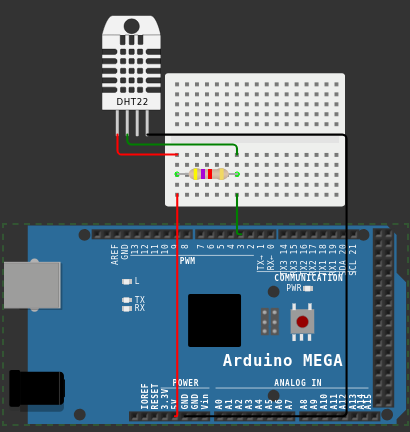
\includegraphics[width=0.7\textwidth]{images/wokwi_dht22_demo.png}
    \caption{Rangkaian sensor DHT22/AM2302 dengan mikrokontroler ATmega2560 pada simulasi Wokwi.}
    \label{fig:dht22_schematic}
\end{figure}

Visualisasi koneksi antarmuka secara lengkap ditunjukkan pada Gambar~\ref{fig:dht22_schematic}, sedangkan rincian pemetaan fungsi pin dan fitur mikrokontroler dirangkum pada Tabel~\ref{tab:dht22_mcu_mapping}.

\begin{table}[H]
	\centering
	\caption{Pemetaan antarmuka DHT22 ke mikrokontroler (ATmega2560)}
	\label{tab:dht22_mcu_mapping}
	\small
	\begin{tabularx}{\textwidth}{@{}lXX@{}}
		\toprule
		Kebutuhan Komponen               & Fitur MCU                      & Alasan Pemilihan \& Fungsi                                                                    \\
		\midrule
		Jalur Komunikasi \textit{1-Wire} & Pin Digital GPIO (misal Pin 2) & Mampu beralih mode dari \textit{Output} (\textit{Start}) ke \textit{Input} (\textit{Data})    \\
		Pengukuran Pulsa Data            & Hardware Timer / Loop Delay    & Membedakan Bit `0' ($26\text{--}28\,\mu\text{s}$) dan Bit `1' ($70\,\mu\text{s}$) via pustaka \\
		Pencegahan \textit{Floating} Bus & External / Internal Pull-Up    & Menjaga bus tetap pada level \textit{HIGH} saat kondisi \textit{idle}                         \\
		\bottomrule
	\end{tabularx}
\end{table}

\paragraph{Kode Demo Pengujian}
Berikut adalah contoh implementasi program sederhana menggunakan pustaka \textbf{Adafruit DHT Sensor Library} pada platform Arduino IDE / Wokwi untuk membaca data temperatur dan kelembapan secara berkala:

\begin{lstlisting}[language=C++, caption={Kode program pembacaan sensor DHT22 pada Arduino/ATmega2560}, label={lst:dht22_code}]
#include <DHT.h>

#define DHTPIN 3       // Pin Digital MCU yang terhubung ke pin DATA DHT22
#define DHTTYPE DHT22  // Menentukan tipe sensor (DHT22/AM2302)

DHT dht(DHTPIN, DHTTYPE);

void setup() {
  Serial.begin(9600);
  Serial.println(F("Pengujian Sensor DHT22/AM2302"));
  dht.begin();
}

void loop() {
  // Jeda minimal 2 detik antar pembacaan (spesifikasi sampling rate DHT22)
  delay(2000);

  float kelembapan = dht.readHumidity();
  float suhu = dht.readTemperature(); // Membaca suhu dalam satuan Celsius

  // Memeriksa jika pembacaan gagal (kembalian NaN)
  if (isnan(kelembapan) || isnan(suhu)) {
    Serial.println(F("Gagal membaca data dari sensor DHT22!"));
    return;
  }

  // Menampilkan hasil pembacaan ke Serial Monitor
  Serial.print(F("Kelembapan: "));
  Serial.print(kelembapan);
  Serial.print(F("%  |  Suhu: "));
  Serial.print(suhu);
  Serial.println(F(" *C"));
}
\end{lstlisting}

\paragraph{Gambaran Hasil Pembacaan}
Setelah kode diunggah ke mikrokontroler atau dijalankan pada simulator Wokwi, keluaran pembacaan data pada \textit{Serial Monitor} akan tampak seperti pada contoh berikut:

\begin{verbatim}
Pengujian Sensor DHT22/AM2302
Kelembapan: 40.00%  |  Suhu: 24.00 *C
Kelembapan: 40.00%  |  Suhu: 24.00 *C
Kelembapan: 40.00%  |  Suhu: 24.00 *C
\end{verbatim}
